\begin{figure}
    \centering
    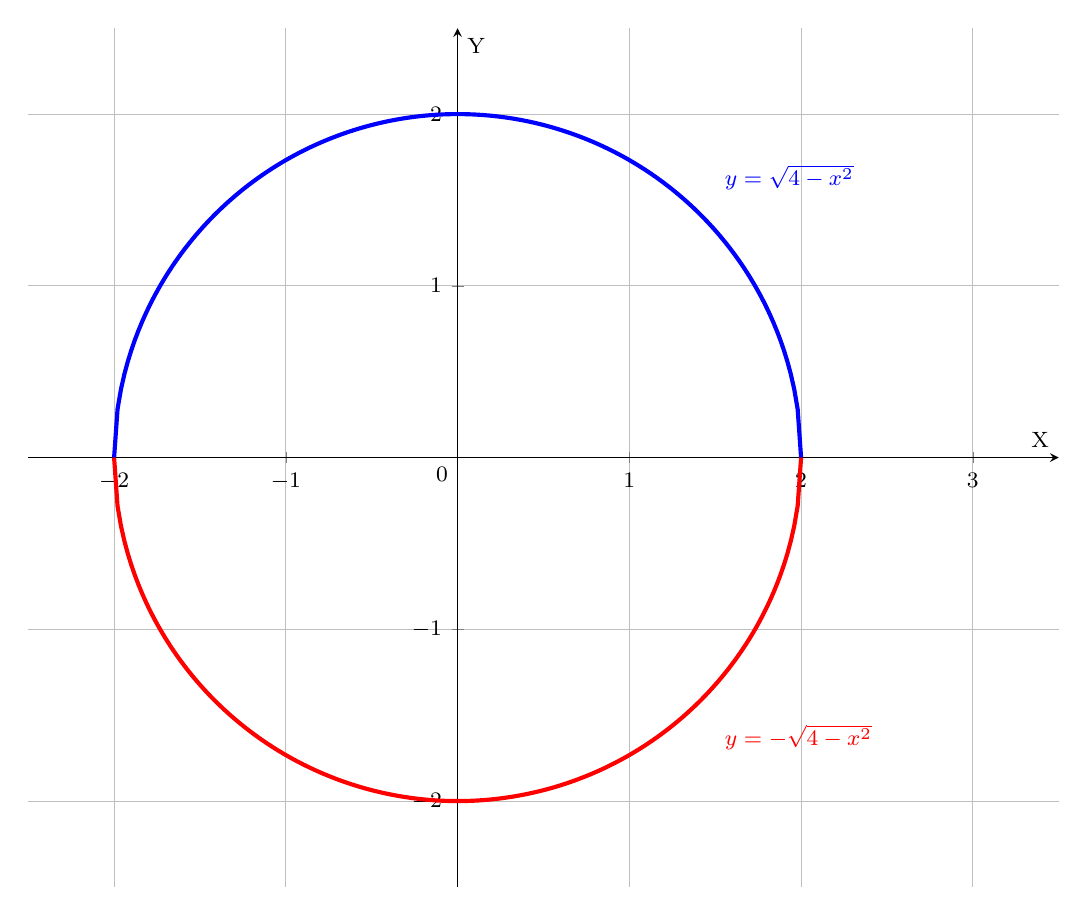
\begin{tikzpicture}
    \begin{axis}[scale=1.5,
            font=\footnotesize,
    	    width=.85\linewidth,
    		xlabel={X},ylabel={Y},
    		xtick = {-3,-2,...,3},
    		ytick = {-3,-2,...,3},
    		xmin=-2.5,xmax=3.5,
    		ymin=-2.5,ymax=2.5,
    		restrict x to domain=-2:3,
    		axis lines=center,
    		grid=both,
    		% grid style={line width=.1pt, draw=gray!10},
      %       major grid style={line width=.2pt,draw=gray!50},
      %       minor tick num=4,enlargelimits={abs=0.5},
    		% axis lines=center,
    		axis equal image,
    		]
    		
    		\node[below left] at (0,0) {$0$};
        	
        	\addplot[domain=-2:2,samples=201,
line width=1.5pt, blue]{sqrt(4-x^2)};
            \addplot[domain=-2:2,samples=201,
line width=1.5pt, red]{-sqrt(4-x^2)};

            \node[above right,blue] at (1.5,1.5) {$y=\sqrt{4-x^2}$};
            \node[below right,red] at (1.5,-1.5) {$y=-\sqrt{4-x^2}$};
    	\end{axis}    
    \end{tikzpicture}
    % \caption{Caption}
    % \label{fig:my_label}
\end{figure}